\documentclass[a4paper,12pt]{article}
\usepackage{float}
\usepackage{pgfplots}
% Preamble: \pgfplotsset{width=1cm,compat=newest}
\begin{document}
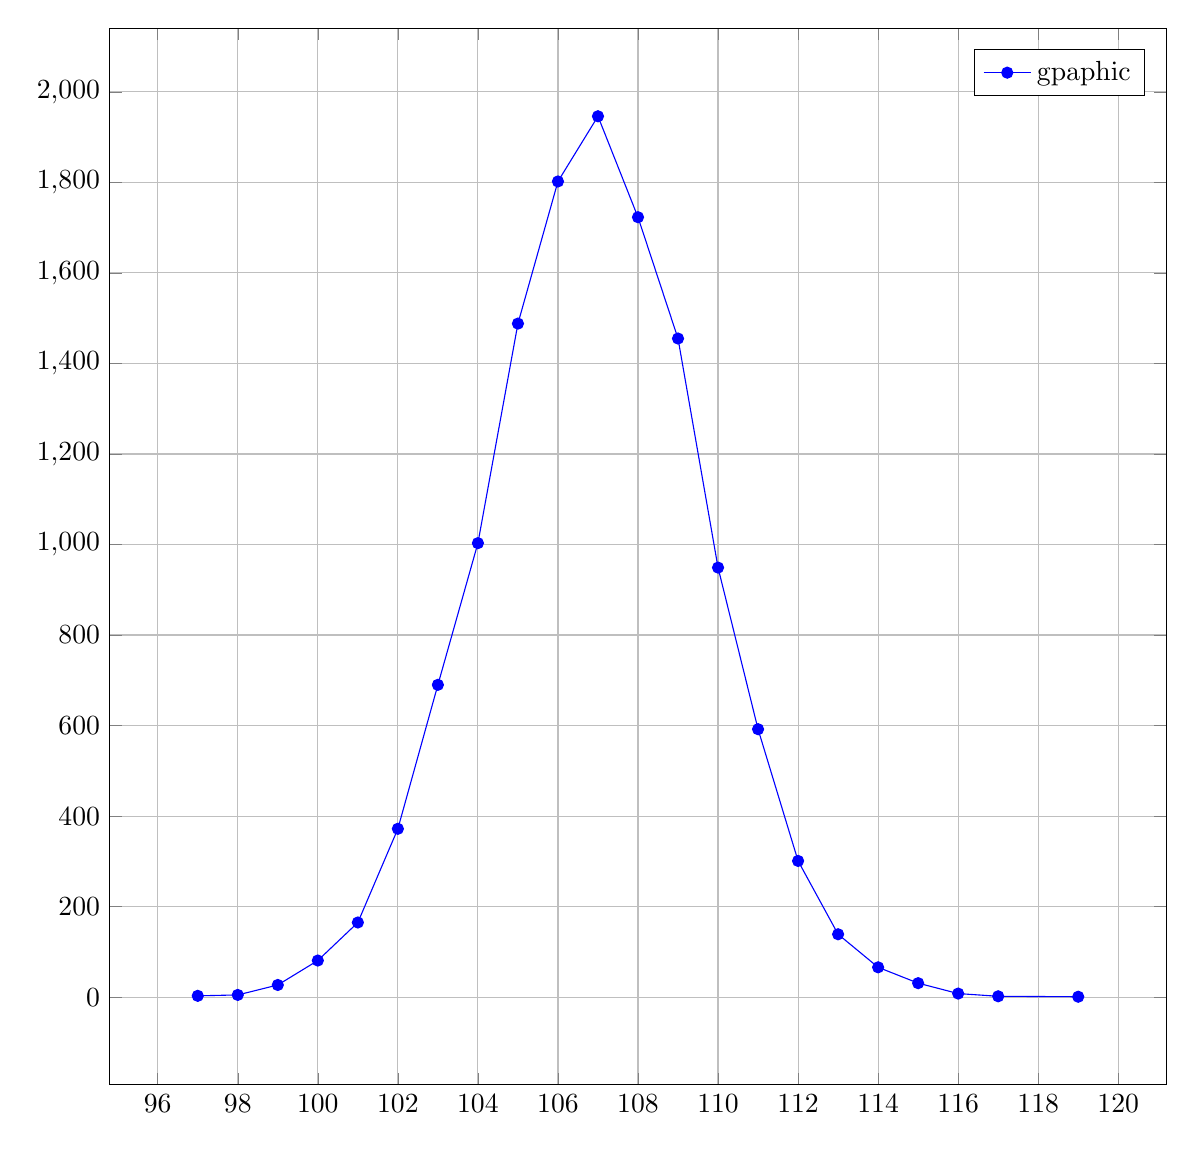
\begin{tikzpicture}
\begin{axis}[height=15cm,width=15cm,grid=major]
\addlegendentry{gpaphic}
\addplot[color = blue, mark = * ] coordinates {
(97,3)
(98,5)
(99,27)
(100,81)
(101,165)
(102,372)
(103,690)
(104,1003)
(105,1488)
(106,1802)
(107,1946)
(108,1723)
(109,1455)
(110,949)
(111,592)
(112,301)
(113,139)
(114,66)
(115,31)
(116,8)
(117,2)
(119,1)
};

\end{axis}
\end{tikzpicture}
\end{document}
